Antes de iniciar cada iteración, el equipo de trabajo revisa las tareas pendientes y además selecciona nuevas tareas que formarán parte del nuevo incremento de funcionalidad, el cual se incorpora al software terminada la iteración. Para realizar lo anterior, se debe tener presente la tecnología y los conocimientos que tiene el equipo para seleccionar los requisitos y así decidir en conjunto, cómo implementar la funcionalidad.

En cuanto al desarrollo, se realiza en la fase del sprint, en donde se satisfacen los requisitos definidos en el sprint backlog dependiendo de la funcionalidad que se debe incorporar en el incremento. Para ello, gran parte del tiempo se desarrolla y revisa antes de incorporar el incremento al proyecto, pero a veces sólo se revisa y ajusta actividades anteriormente realizadas ante algún cambio que surge tras las entregas de los incrementos. Posteriormente, pasa por un proceso de revisión para verificar si el incremento cumple con lo requerido. Todo lo mencionado con anterioridad se repiten en iteraciones que duran aproximadamente 30 días a lo largo del proyecto hasta culminar con el producto. Cabe destacar que cuando se comienza un sprint, no se pueden agregar nuevos cambios. Por lo tanto, esto permite trabajar en un ambiente enfocado a corto plazo, pero estable. En resumen, la \textbf{Figura~\ref{fig: procesoScrum}} muestra las fases que se mencionaron de forma general.

\begin{figure}[h!]
    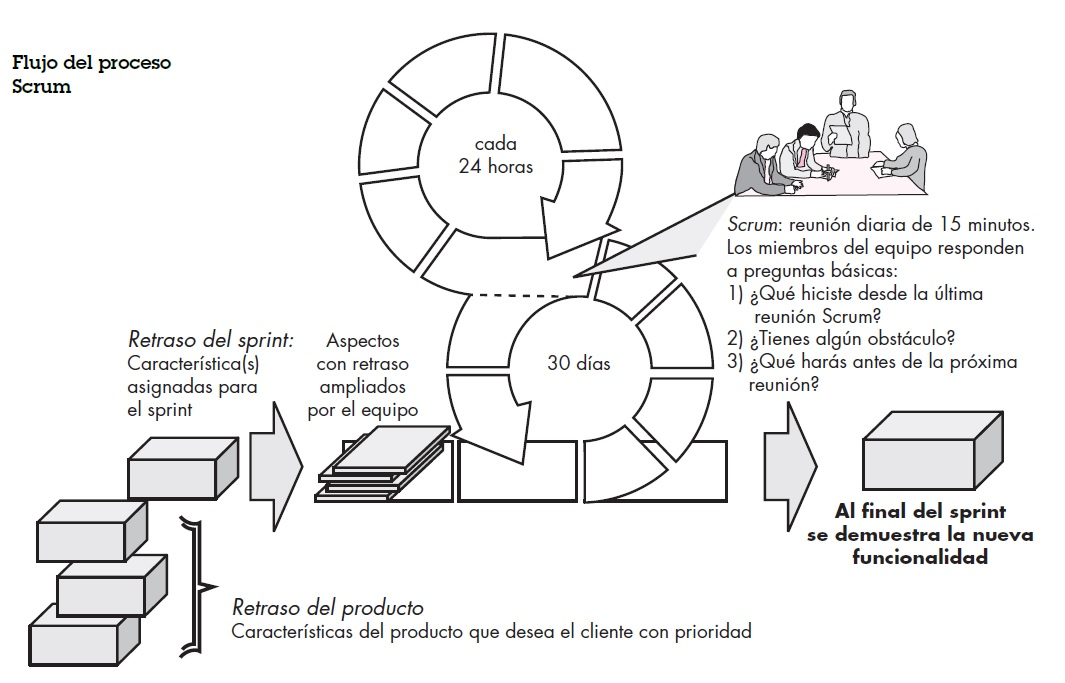
\includegraphics[width=\textwidth]{Imagenes/Scrum.jpg}
    \caption{\label{fig: procesoScrum} Proceso de metodología Scrum.}
\end{figure}